\chapter{Appendix}

\section{Appendix 1}
\begin{table}[h!] \label{}
\caption{All of the used parameters and their meaning and values}
\label{tab:Params}
\centering
\resizebox{\textwidth}{!} {%
\begin{tabular}{@{}llll@{}}
\toprule
Symbol       & Interpretation           & Units     & Value     \\ \midrule
\multicolumn{4}{@{}l}{\textbf{\textit{Independent variables}}}              \\
t            & Time                     & $d$         & -         \\
z            & Depth                    & $m$         & -         \\
\multicolumn{4}{@{}l}{\textbf{\textit{Dependent variables}}}                \\
P(z,t)       & Phytoplankton density    & $cells/m^3$ &           \\
N(z,t)       & Nutrient concentration   & $mmol \: nutrient/m^3$  &  \\
I(z,t)       & Light intensity          & $\mu mol \: photons/m^{2} d$ &  \\
$I_{surface}(t)$ & Incident light at surface & $\mu mol \: photons/m^{2} d$ & \\
\multicolumn{4}{@{}l}{\textbf{\textit{Parameters}}}                         \\
$I_0$          & Annual average incident light at surface & $\mu mol \: photons/m^{2} d$ & 2.592e07  \\
$k_w$          & Turbidity of water & $m^{-1}$               & 0.045     \\
$k_P$          & Attenuation coefficient of phytoplankton  & $m^{2}/cell$ & 6.000e-10 \\
$H_I$          & Half-saturation constant of light limited growth & $\mu mol  \: photons/m^{2} d$ & 2.592e06  \\
$H_N$          & Half-saturation constant of nutrient limited growth & $mmol \: nutrient/m^3$  & 0.0425    \\
D            & Diffusivity  & $m^{2}/d$              & 30        \\
u            & Advection (sinking velocity)  & $m/d$ & 1         \\
l            & Mortality / loss rate   & $d^{-1}$     & 0.240     \\
$\alpha$     & Nutrient content of a phytoplankton cell & $mmol \: nutrient/cell$ & 1.00e-09  \\
$\varepsilon$  & Nutrient recycling coefficient  & $dimensionless$ & 0.5       \\
$N_B$  & Nutrient concentration at the bottom & $mmol \: nutrient/m^3$  & 10    \\
$\mu_{max}$         & Maximum growth rate   & $day^{-1}$    & 0.960     \\
$I_{amplitude}$  & Amplitude of seasonal variation in incident light       & $\mu mol \: photons/m^2 d$ & 2.592e07  \\
$\phi$          & Latitude used for seasonal variation in light intensity & $Degrees$            & 55        \\ \bottomrule
\end{tabular}%
}
\end{table}

\newpage
\section{Appendix 2}
\begin{figure}[!htb]
\centering
\begin{subfigure}{.8\textwidth}
  \centering
  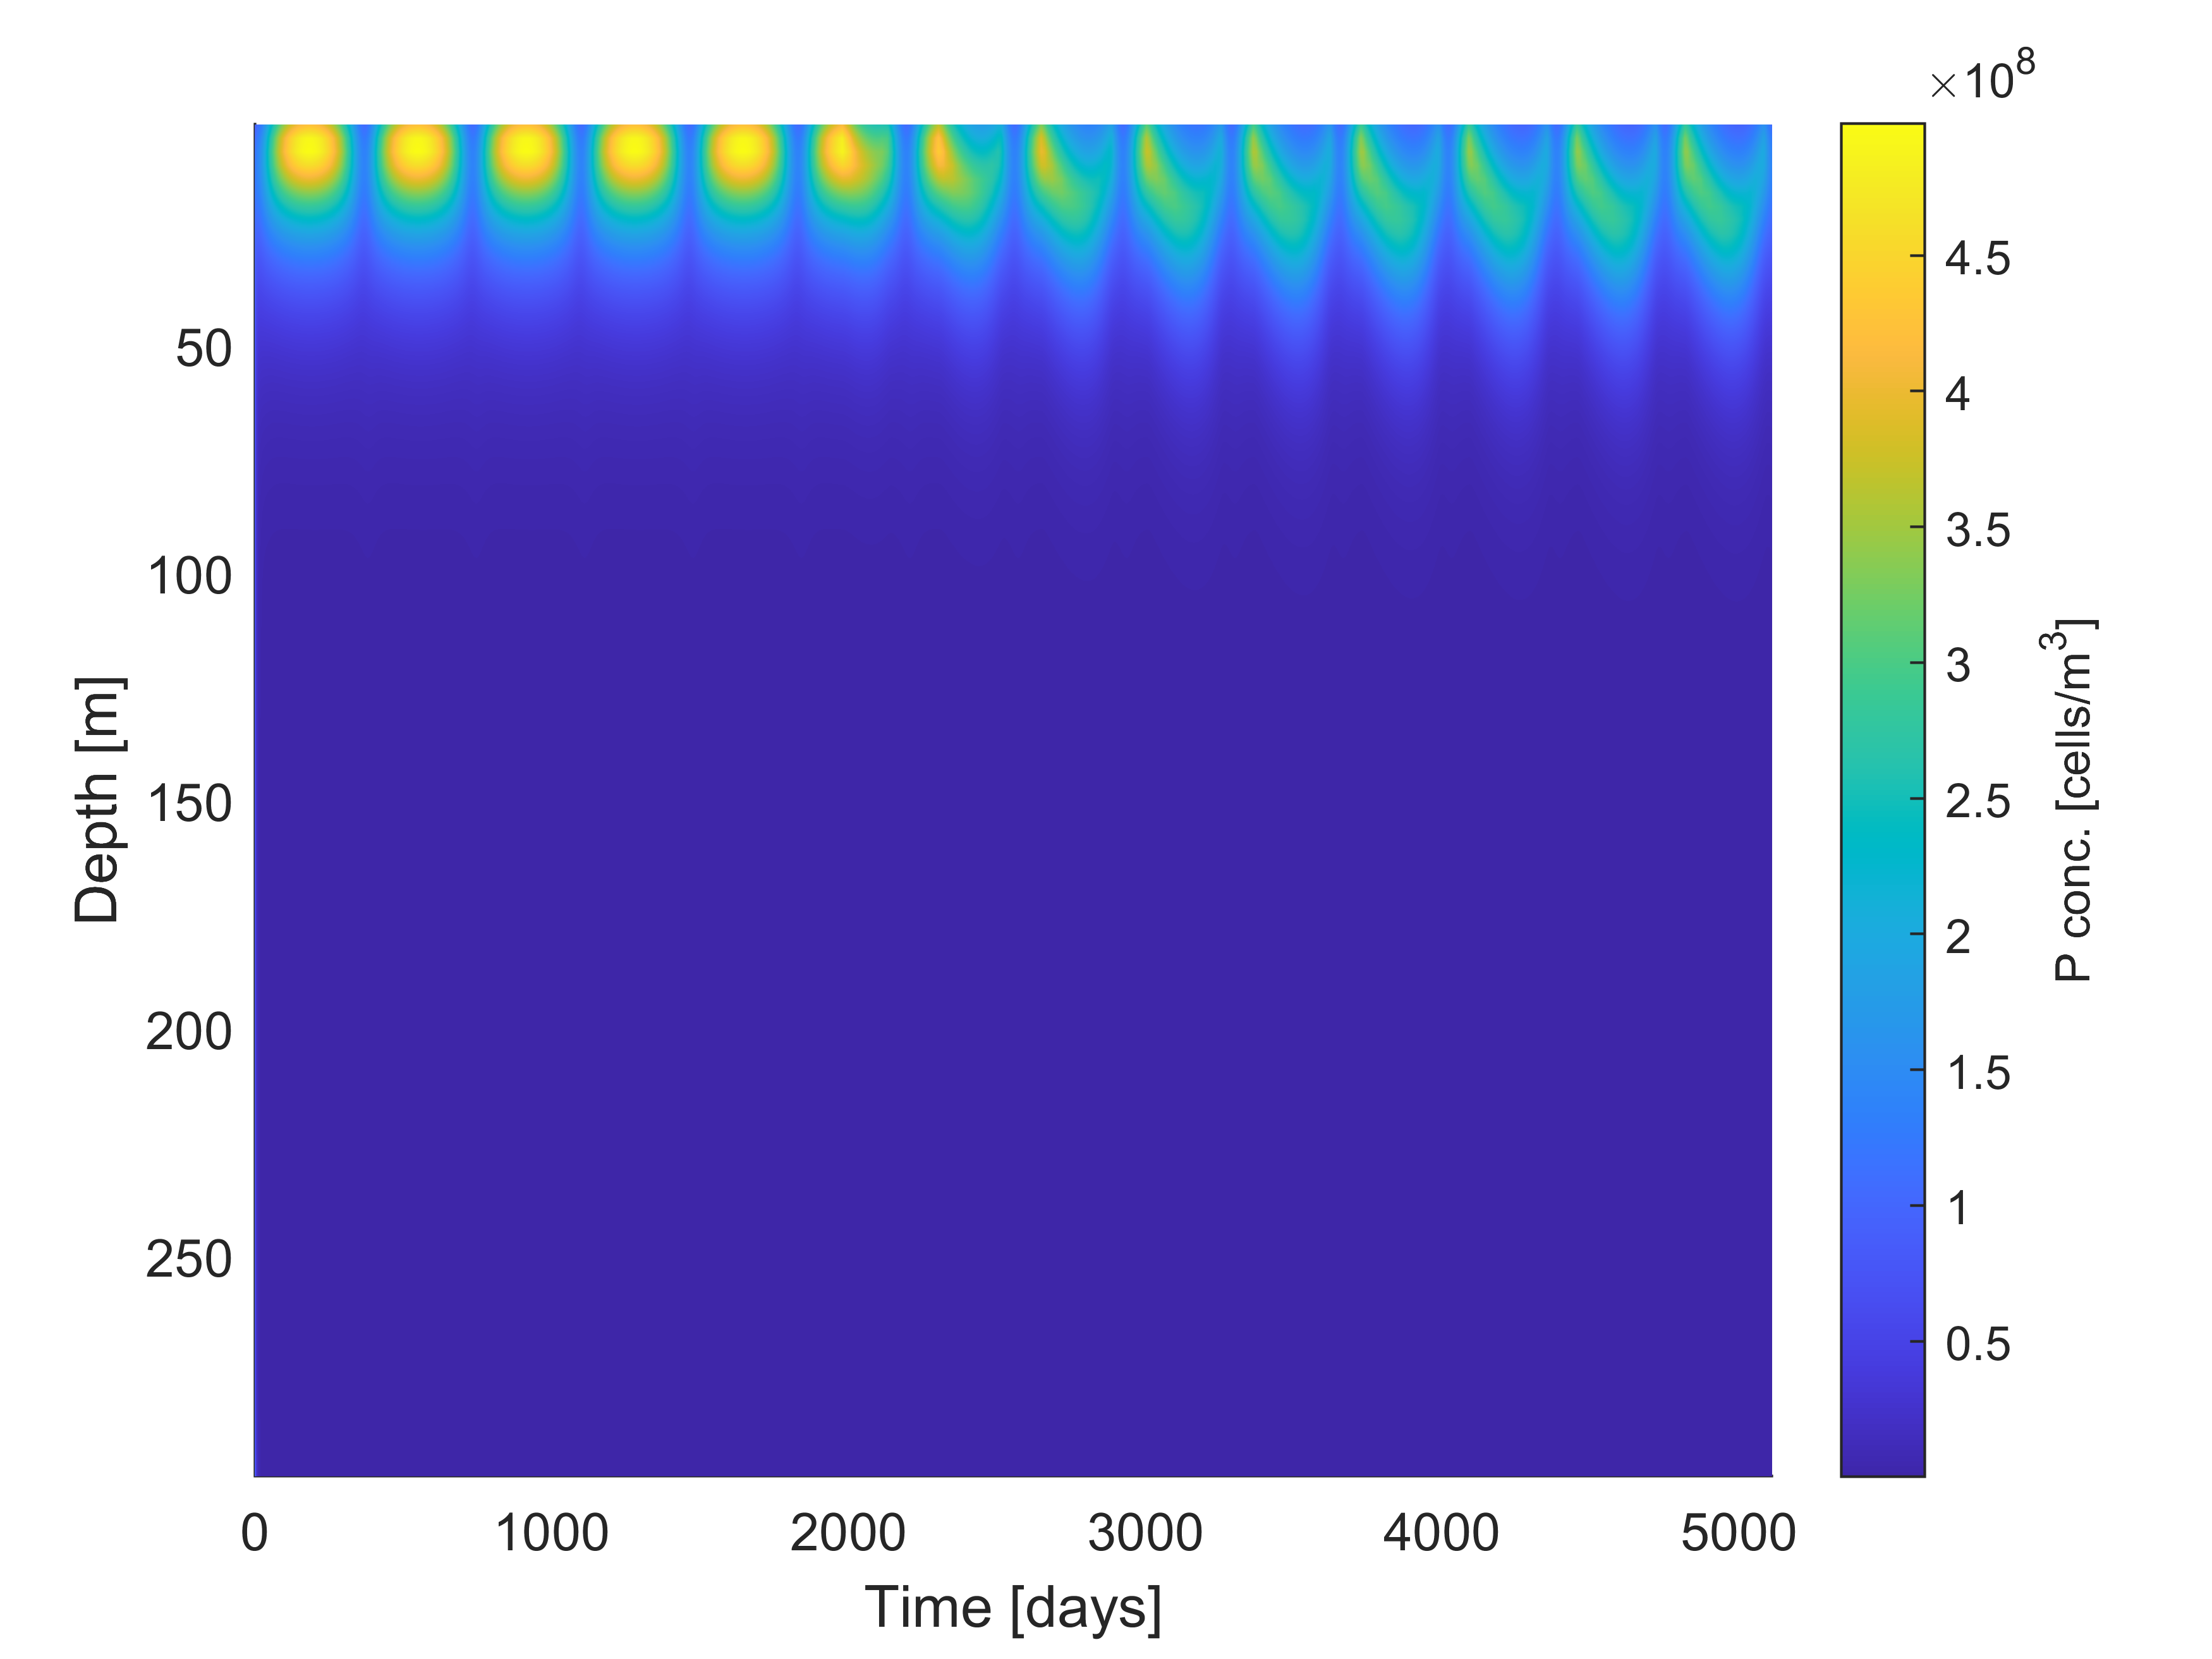
\includegraphics[width=\linewidth]{Pictures/Baserun_P.png}
  \caption{3D plot of pythoplankton}
  \label{fig:baserunP}
\end{subfigure}%

\begin{subfigure}{.8\textwidth}
  \centering
  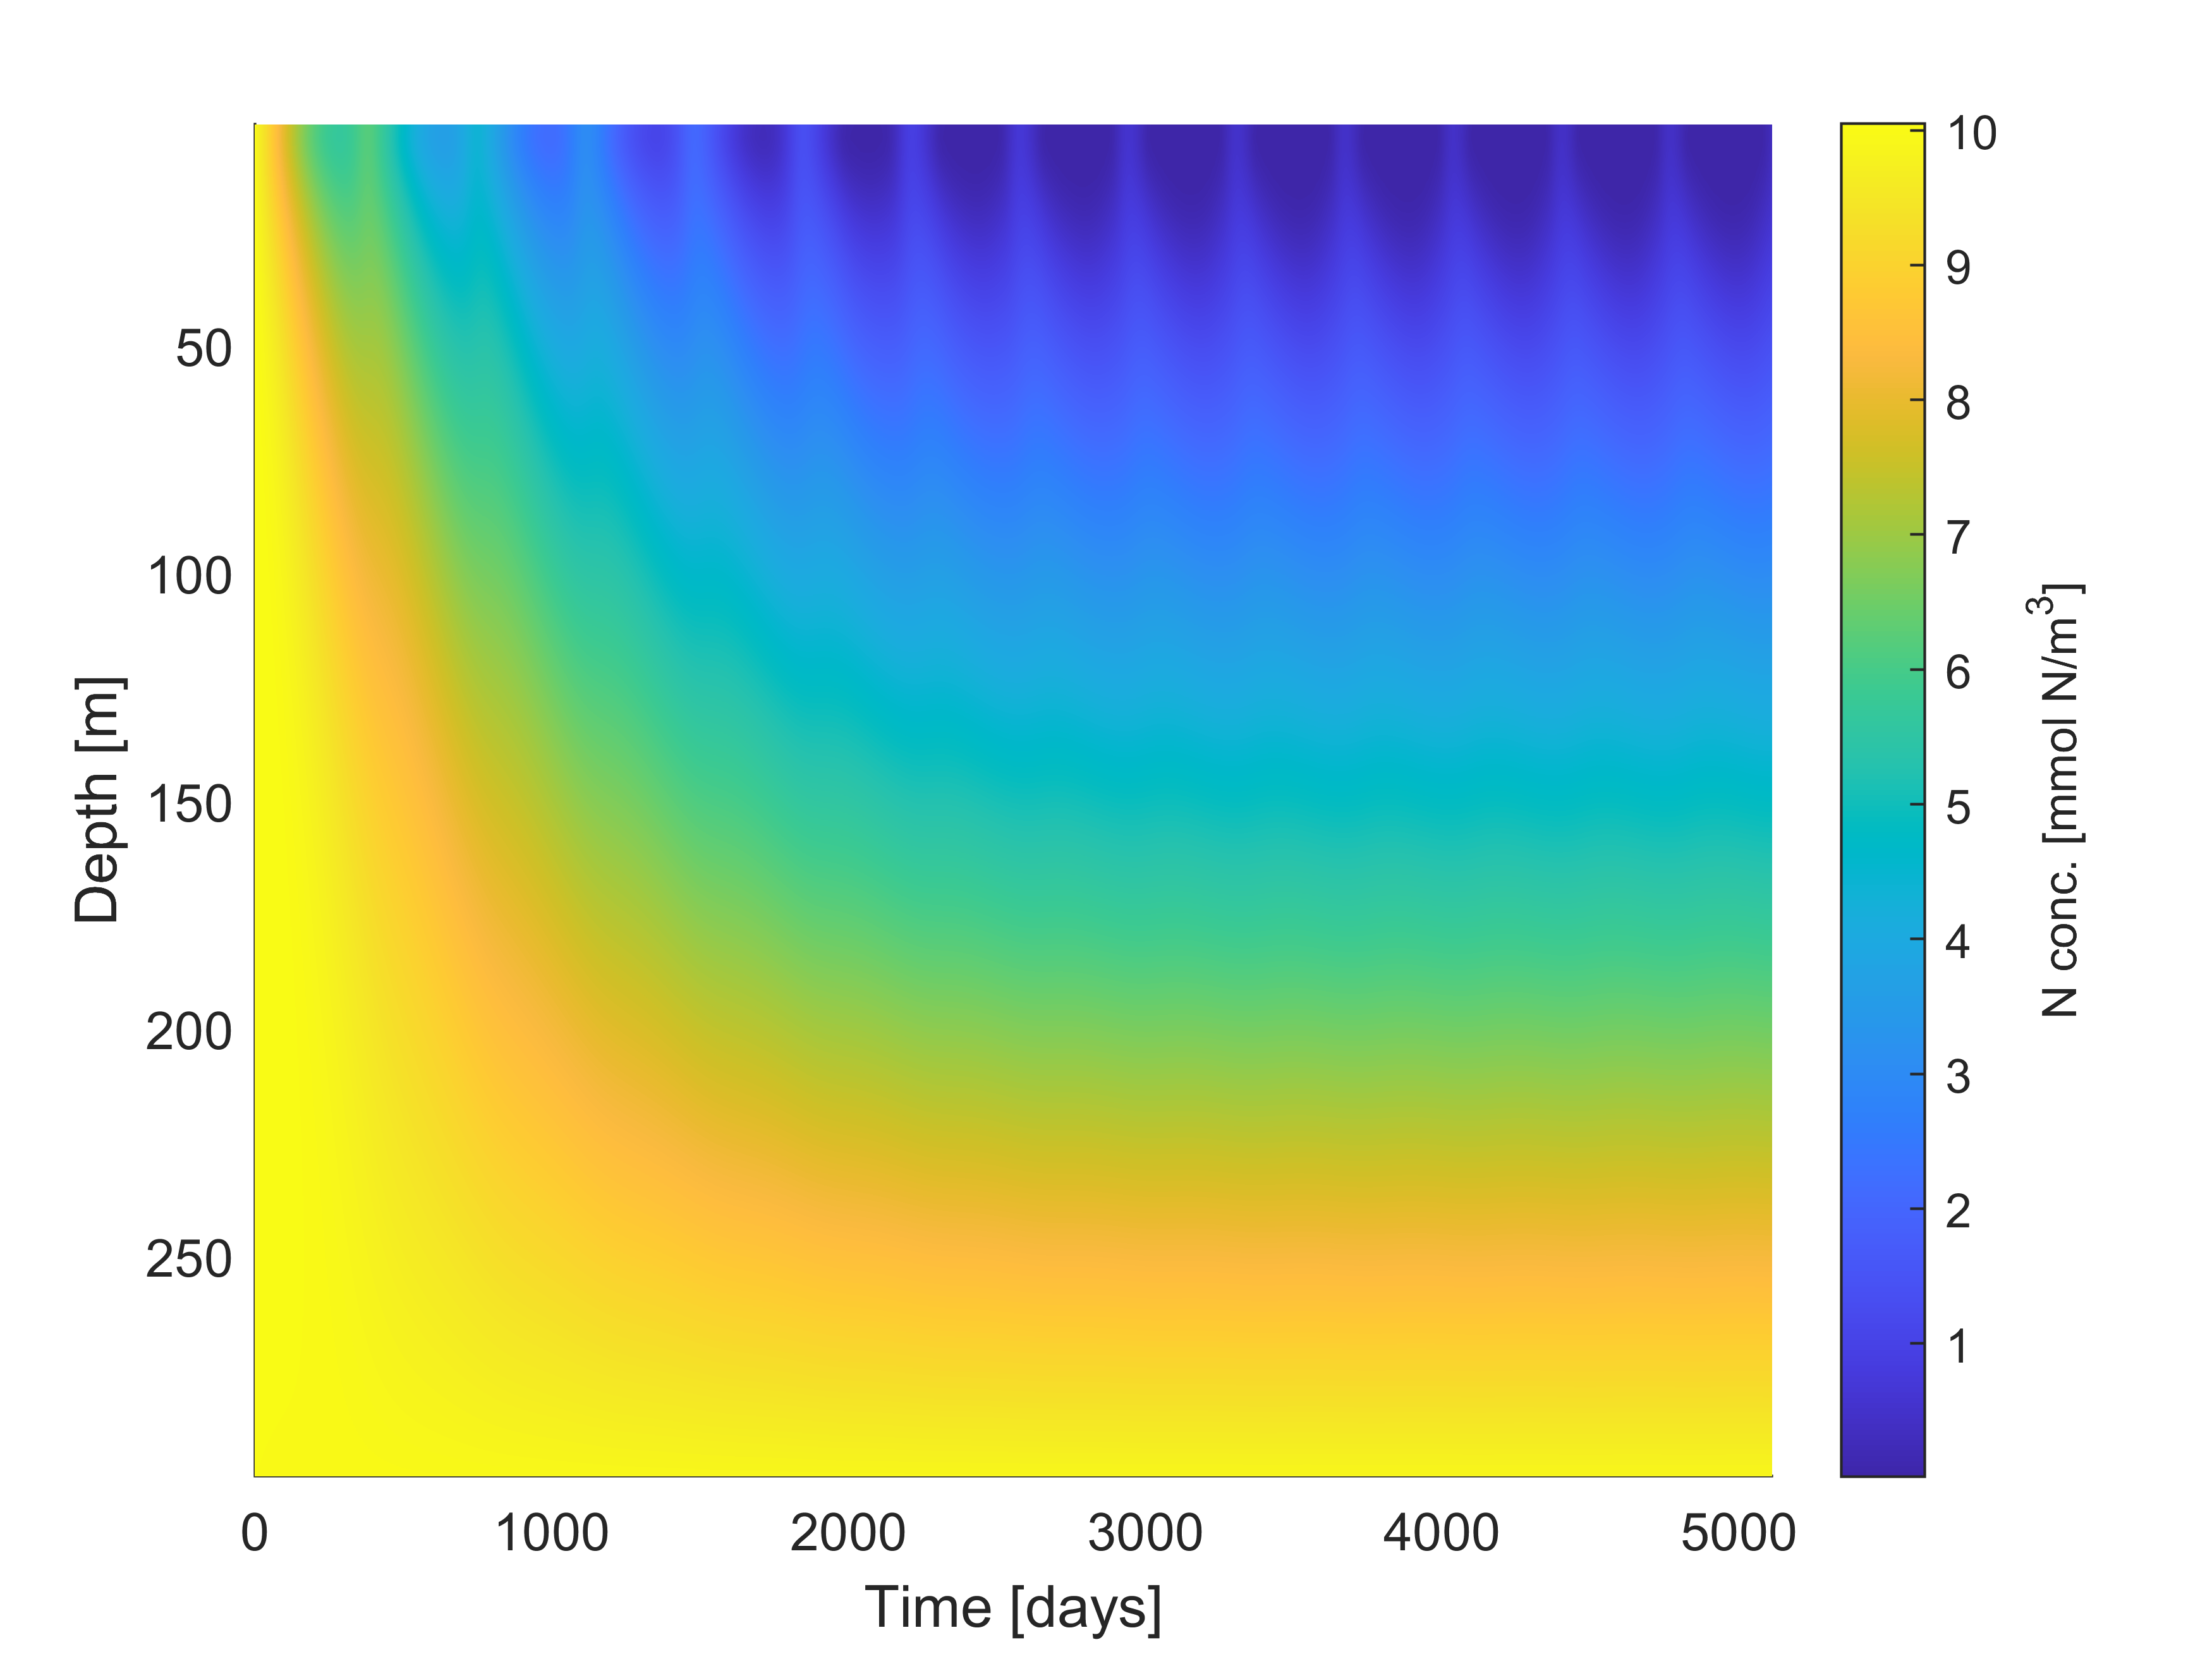
\includegraphics[width=\linewidth]{Pictures/Baserun_N.png}
  \caption{3D plot of nutrients}
  \label{fig:baserunN}
\end{subfigure}
\caption{The model derived solutions for 14 years [5110 days] for both P (a) and N (b) plotted in 3D plots}
\label{fig:baserunplots}
\end{figure}

\section{Appendix 3}
\begin{lstlisting}[language=Matlab, caption = baserun.m - used to run the model and get results in a struct called res]
close all
clear all
%% Run the model and get results in the res-struct:
res = NPD(param);

plotNPD(res, param)
\end{lstlisting}

\section{Appendix 4}
\begin{lstlisting}[language=Matlab, caption = NPD.m - the body of the model that calculates the derivative of the ODEs]
function res = NPD(param)

%Initial conditions:
P0 = linspace(0,0, param.depth/param.dz);
P0(1:length(P0)) = 1e08;          %Initial concentration
N0 = linspace(0,0, param.depth/param.dz);
N0(1:length(P0)) = 10;          %Initial concentration

%Time range:
tRange = [0:5110]; %tRange - time range in days

%Run the model:
[t, y] = ode45(@derivative, tRange, [N0 P0], [], param);

z = param.z; % i dont know what this is for

%Assemble results:
res.N = y(:,1:param.nGrid);
res.P = y(:,(param.nGrid+1):(2*param.nGrid));
res.z = z;
res.t = t;
res.p = param;
res.Plast = res.P(end,:);
%res.light = I_light;
[res.maxvalue, res.index] = max(res.Plast);
res.zAtIndex = res.z(res.index);

%----------------- derivative function: ---------------------%

    function dydt = derivative(t,y, param)
        N = y(1:param.nGrid);
        P = y((param.nGrid+1):(2*param.nGrid));
        
        ix = 2:(param.nGrid);
        
        %%%%%%%%%%%%%%%%%%%%%%%%%%%%%%%%%%%%%%%%%%%
        %------------ Nutrients: -----------------%
        %%%%%%%%%%%%%%%%%%%%%%%%%%%%%%%%%%%%%%%%%%%
        JdN(ix) = -param.D*(N(ix)-N(ix-1))/param.dz; %Diffusivity of N
        
        % Boundary conditions for JdN:
        JdN(1) = 0; % No flux at the surface...
        JdN(param.nGrid+1) = -param.D*(param.NB-N(end))/param.dz;

        %%%%%%%%%%%%%%%%%%%%%%%%%%%%%%%%%%%%%%%%%%%
        %---------- Phytoplankton: ---------------%
        %%%%%%%%%%%%%%%%%%%%%%%%%%%%%%%%%%%%%%%%%%%        
        %-------- P_Advective fluxes: ---------------%
        JaP(ix) = param.u*P(ix-1);
        %Boundary conditions for Ja:
        JaP(1) = 0;  % No input from the surface
        JaP(param.nGrid+1) = 0; % Closed bottom
        
        %---------- P_Diffusive fluxes: -------------------%
        JdP(ix) = -param.D*(P(ix)-P(ix-1))/param.dz;
        
        % Boundary conditions for Jd:
        JdP(1) = 0; % No flux at the surface...
        JdP(param.nGrid+1) = 0;  % ...or the bottom
        
        %---------- Reaction term / division rate: -------------------%
        % Calculate light:
        I_light = zeros;
        I_light = calclight(P, t, param);
        
        % Calculate division rate:
        mu(ix) = param.mumax*min((N(ix)'./(param.HN+N(ix)')),(I_light(ix)./(param.HI+I_light(ix))));
        
        
        % ----------- wrapping up and calculate dPdt: ------------%
        % Calculate Rate-of-change due to advection, diffusion and reaction:
        JP = JaP + JdP; %total flux for phytoplankton
        JN = JdN;
        
        %Calculate dNdt:
        dNdt = zeros;
        dNdt = -param.a.*mu.*P'+param.e*param.a*param.l.*P'-(JN(2:(param.nGrid+1))-JN(1:param.nGrid))/param.dz;
        %Calculate dPdt:
        dPdt = zeros;
        dPdt = -(JP(2:(param.nGrid+1))-JP(1:param.nGrid))/param.dz + mu.*P'- param.l.*P';
        
        % Make dPdt a column vector:
        dydt = [dNdt dPdt]';
    end
end 
\end{lstlisting}

\section{Appendix 5}
\begin{lstlisting}[language=Matlab, caption = calclight.m - used to calculate the seasonality of surface incident light and the light intensity throughout the water column]
% Calculating light:
function I = calclight(P, t, param)
Isurface = param.I0-param.Iamplitude*sin((pi*55)/180).*cos(2*pi.*(t/365));
I = Isurface*exp(-param.kw*param.z-param.kp*cumsum(P)*param.dz);

%I = param.I0*exp(-param.kw*param.z-param.kp*cumsum(P)*param.dz); %used
%when seasonality is excluded
end
\end{lstlisting}

\section{Appendix 6}
\begin{lstlisting}[language=Matlab, caption = param.m - a function collecting all parameter values used in the model]
function param = param()
% Parameter construct:
param.D         = 30;           %Diffusion (UML) [m2 day-1]
param.u         = 1;            %Advection velocity [m day-1]
param.HI        = 30*86400;     %half saturation constant of light limited growth [µmol photons m-2 day-1]
param.HN        = 0.0425;       %half saturation constant of nutrient limited growth [µmol photons m-2 day-1]
param.kp        = 6*10^-10;     %Specific light attenuation for plankton [m2 cell-1];
param.kw        = 0.045;        %Background water turbidity [m-1]
param.I0        = 300*86400;    %Incident Light intensity [µmol photons m-2 day-1]
param.Iamplitude = 300*86400;   %Used to calculate seasonality in calclight.m;
param.l         = 0.01*24;      %specific loss rate [day-1]
param.mumax     = 0.04*24;      %maximum specific growth rate [day-1]
param.a         = 1*10^-9;      %Nutrient content of phytoplankton [mmol nutrient/cell]
param.e         = 0.5;          %Nutrient recycling coefficient
param.NB        = 10; %Nutrient conc. at the bottom


%Grid properties:
param.depth     = 300;                  %Depth [m]
param.dz        = param.depth/100;      %grid spacing [m]
param.z         = param.dz/2:param.dz:(param.depth-param.dz/2); % center of each grid
param.nGrid     = length(param.z);  % No. of grid cells
end
\end{lstlisting}

\section{Appendix 7}
\begin{lstlisting}[language=Matlab, caption = plotNPD.m - used to make most of the plots shown in this report]
function plotNPD = plotNPD(res, param)
    close all
    % Plot the model results:
    figure(1)
    surface(res.t,res.z,res.P')
    shading interp
    xlabel('Time [days]')
    ylabel('Depth [m]')
    axis ij
    axis tight
    cb1 = colorbar;
    cb1.Label.String = 'P conc. [cells/m^3]';
    %title('Phytoplankton')

    figure(2)
    surface(res.t,res.z,res.N')
    shading interp
    xlabel('Time [days]')
    ylabel('Depth [m]')
    axis ij
    axis tight
    cb2 = colorbar;
    cb2.Label.String = 'N conc. [mmol N/m^3]';
    %title('Nutrients')

    % --------------- max(P) plot ---------------
    figure(4)
    plot(res.zAtIndex, res.maxvalue, 'b*')
    xlabel("depth [m]")
    ylabel("Max P at t=2000")

    %---------------- light/nutrient limitation
    N = res.N(4746,:); %jan 1st of year 14.
    P = res.P(4746,:);
    t = res.t(4746);
    HN = res.p.HN;
    HI = res.p.HI;

    I = calclight(P, t, param);

    for i = 1:length(N)
        N_lim(i) = N(i)/(HN+N(i));
        I_lim(i) = I(i)/(HI+I(i));
    end
    figure(5)
    plot(N_lim, -res.z)
    hold on
    plot(I_lim, -res.z)
    xline(param.l/param.mumax, 'k--')
    xlabel('Growth limiting terms')
    ylabel('Depth [m]')
    ylim([-100 0])
    legend('N/(N+H_N)', 'I/(I+H_I)','l/µmax', 'Location', 'South')
    
    figure(9)
    plot(P,-res.z)
    xlabel('P conc. [cells/m^3]')
    ylabel('Depth [m]')
    ylim([-100 0])
    
    figure(6)
    t1 = [1:365];
    plot(t1, (param.I0-param.Iamplitude*sin((pi*55)/180).*cos(2*pi.*(t1/365))))
    hold on
    yline(param.I0, 'r-')
    hold off
    xlabel('Day of the year')
    xlim([0 365])
    ylabel('Incidient light at the surface [µmol photons/m^2 d]')
    legend('Incident light at surface', 'Annual average incident light (I_0)','Location', 'south')
    
    figure(7)
    plot(I, -res.z, 'k-') %January 1st year 14
    P = res.P(4846,:); %april 10th year 14
    t = res.t(4846);
    I2 = calclight(P, t, param);
    hold on
    plot(I2, -res.z, 'r-')
    P = res.P(4946,:); %july 19th year 14
    t = res.t(4946);
    I3 = calclight(P, t, param);
    plot(I3, -res.z, 'b-')
    xlabel('Light intensity [µmol photons/m^3]')
    ylabel('Depth [m]')
    ylim([-75 0])
    legend('I at Jan. 1 year 14', 'I at April 10th year 14', 'I at July 19th year 14', 'Location', 'southeast')
    
    figure(8)
    plot(res.P(end,:),-res.z)
    
    figure(11)
    plot(res.P(4746,:), -res.z, 'k-') %January 1st year 14
    hold on
    plot(res.P(4846,:), -res.z, 'r-') %april 10th year 14
    plot(res.P(4946,:), -res.z, 'b-') %july 19th year 14
    plot(res.P(5046,:), -res.z, 'g-') %October 27th year 14
    xlabel('P conc. [cells/m^3]')
    ylabel('Depth [m]')
    ylim([-150 0])
    legend('P at Jan. 1 year 14', 'P at April 10th year 14', 'P at July 19th year 14','P at Oct. 27th year 14', 'Location', 'southeast')
    
    figure(12)
    surface(res.t((4746:end),:),res.z,res.P((4746:end),:)')
    shading interp
    xlabel('Time [days]')
    ylabel('Depth [m]')
    axis ij
    axis tight
    cb1 = colorbar;
    cb1.Label.String = 'P conc. [cells/m^3]';
    
    figure(13)
    surface(res.t((4746:end),:),res.z,res.N((4746:end),:)')
    shading interp
    xlabel('Time [days]')
    ylabel('Depth [m]')
    axis ij
    axis tight
    cb1 = colorbar;
    cb1.Label.String = 'N conc. [mmol N/m^3]';
\end{lstlisting}